{\small
\section{Stream-API $\qquad\qquad$ java.util.stream.*}
    \begin{tabular}{l}
        $\bullet$ Wird für deklarative Abfragen von Collections gebraucht\\
        $\bullet$ Code definiert, \textbf{was} gesucht wird, nicht \textbf{wie}\\
        $\bullet$ Framework arbeitet sehr intensiv mit Lambdas\\
        $\bullet$ Ist komplett unabhängig von Input/Output-Streams\\    
    \end{tabular}

    \begin{tabular}{l l}
        \rowcolor[RGB]{239,239,239} 
        \textbf{Basisschnittstellen} $\qquad$ & \textbf{Für primitive Datentypen}\\
        $\bullet$ \verb|Stream<T>| &$\bullet$ \verb|IntStream|\\
        & $\bullet$ \verb|LongStream|\\
        & $\bullet$ \verb|DoubleStream|\\
    \end{tabular}
    \vspace{-0.3cm}

\subsection{Endliche Quellen}
    \begin{tabular}{l l}
        \verb|list.stream()              | & Liefert Stream anh. Collection \\
        \verb|Arrays.stream(array)       | & Liefert Stream anh. Array \\
        \verb|IntStream.range(1, 100)    | & Zahlen von 1 bis 100 \\
        \verb|Stream.of(2, 3, 5, 7)      | & eigene Aufzählung \\
        \verb|Stream.concat(strm1, strm2)| & Verketteter Stream \\
    \end{tabular}
    \vspace{-0.3cm}

\subsection{Unendliche Quellen}
    \begin{minipage}{0.5\linewidth}
        \verb|generate()| \\
        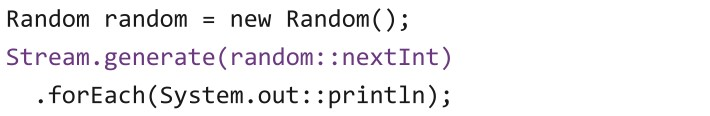
\includegraphics[width=1.2\linewidth]{pictures/generate.jpg}
    \end{minipage}
    \hfill
    \begin{minipage}{0.5\linewidth}
        \verb|iterate()| \\
        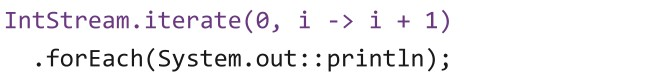
\includegraphics[width=1.2\linewidth]{pictures/iterate.jpg}
    \end{minipage}
    \vspace{-0.3cm}

\subsection{Zwischenoperationen}
    \begin{tabular}{l l}
        \verb|filter(Predicate) | & Filtern mit Lambda \\
        \verb|map(Function)     | & Mappen mit Lambda \\
        \verb|mapToInt(Function)| & Mappen mit \verb|int,long, double| \\
        \verb|sorted(Comparator)| & Sortieren mit Comparator \\
        \verb|distinct()        | & Duplikate entfernen gemäss \verb|equals()| \\
        \verb|limit(long n)     | & n-Elemente liefern \\
        \verb|skip(long n)      | & n-Elemente überspringen \\
    \end{tabular}

    Zwischenoperationen dürfen die Collection \textbf{nicht ändern} und sie dürfen keine Abhängigkeit zu äusseren, änderbaren Variablen haben.
    \vspace{-0.3cm}

\subsection{Terminaloperationen (beenden Stream)}
    \begin{tabular}{l l}
        \verb|forEach(Consumer)     | & Pro Element Operation anwenden \\
        \verb|count()               | & Anzahl Elemente \\
        \verb|min(),max()           | & bei \verb|Stream<T>| Comparator-Arg. erf. \\
        \verb|average(), sum()      | & Nur bei in/long/double-Stream \\
        \verb|findAny(), findFirst()| & Gibt irgendein/erstes Element zurück \\
        \verb|collect()|              & Rückumwandlung zu Collection \\
        \verb|toArray()|              & Rückumwandlung zu Array \\
    \end{tabular}
    \vspace{-0.3cm}

    \subsubsection{Collectors $\rightarrow$ collect(...)}
        \verb|Collectors.toList()| $\rightarrow$ in Liste abbilden

        \verb|Collectors.toCollection(TreeSet::new)| \\
        $\hookrightarrow$ in beliebige Collection abbilden (Konstruktorreferenz)

        \verb|Collectors.groupingBy(key, aggregator)|:

        \begin{tabular}{l}
            $\bullet$ Gruppierung mit opt. Aggregator\\
            $\bullet$ Aggregator: averaging, summing, counting\\
            $\bullet$ Liefert HashMap als Rückgabewert\\
        \end{tabular}
        \vspace{-0.3cm}

\subsection{Funktionsschnittstellen}
    \subsubsection{Vordefinierte}
        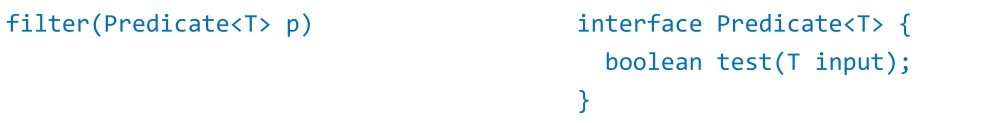
\includegraphics[width=0.8\linewidth]{pictures/funktionsschnitt-vordef_1.jpg}
        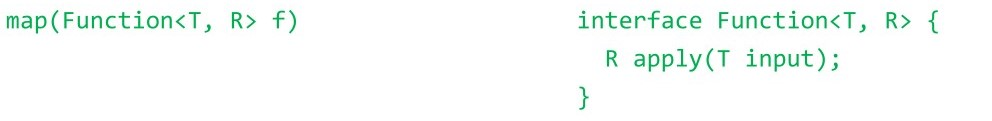
\includegraphics[width=0.8\linewidth]{pictures/funktionsschnitt-vordef_2.jpg}
        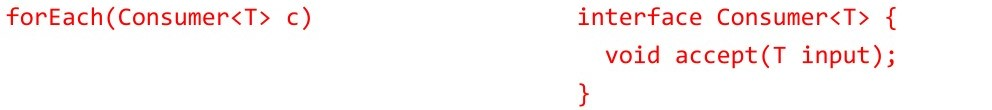
\includegraphics[width=0.8\linewidth]{pictures/funktionsschnitt-vordef_3.jpg}
        \vspace{-0.3cm}

    \subsubsection{Optional-Wrapper}
        \verb|average(), min(), max(), findAny(), findFirst()| \\
        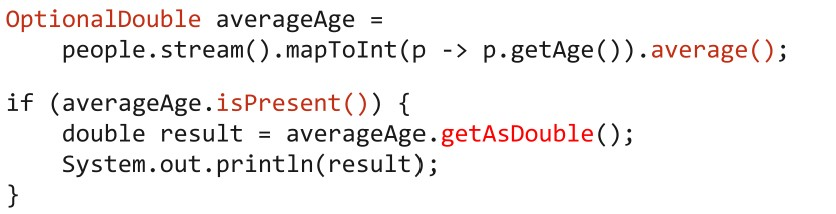
\includegraphics[width=0.8\linewidth]{pictures/optional-wrapper.jpg}
        \vspace{-0.3cm}

    \subsubsection{Matching}
        \verb|allMatch(), anyMatch(), noneMatch()| \\
        Prüfen, ob das Prädikat auf alle / irgendein/ kein Element zutrifft \\
        \verb|boolean 18plus = ppl.stream().allMatch(p->p.getAge >= 18);|
        \vspace{-0.2cm}

}